\section{Aufgabe 1} \label{sec:ab}
\subsection{Teilaufgaben a und b)}
Für die Funktionen
\begin{align}
  f(x)=\left(x^3+\frac{1}{3} \right)-\left(x^3-\frac{1}{3}\right ) \label{eqn:f}\\
  g(x)=\frac{\left(3+x^3 \right)-\left(3-x^3\right )}{x^3} \label{eqn:g}
\end{align}
sollte empirisch ein Bereich bestimmt werden, in denen sie um nicht mehr als 1\% abweichen.
Dazu wurde die Funktion "check" in Aufgabe01.py geschrieben. Diese nimmt, unter Anderem, einen Anfangs- und Grenzwert und überprüft, ab welchem
$x$ die Funktionen um 1\% abweichen.
Dabei ergaben sich folgende Ausgaben:
\begin{console1}{ für \eqref{eqn:f}}
  Fuer ein x von 0 bis 180000 mit 0 Dezimalstellen ergeben sich folgende Abweichungen: \\
  x=41286  f(x)=0.65625, Fehler : 1.5625\% \\

  Zusaetzlich ergibt sich als Nullstelle: \\
  x=165141f(x)=0.0, Fehler : 100.0\% \\
\end{console1}
\begin{console1}{ für \eqref{eqn:g}}
  Fuer ein x von 1 bis 0 mit 8 Dezimalstellen ergeben sich folgende Abweichungen: \\
  x=4.013000000002709e-05  f(x)=0.6734243528892833, Fehler : 1.0136529333924837 \% \\

  Zusaetzlich ergibt sich als Nullstelle: \\
  x=8.730000000012339e-06f(x)=0.0, Fehler : 100.0 \% \\

\end{console1}
Die zu untersuchenden Bereiche wurden bewusst so gewählt.
\begin{itemize}
  \item der Term $x^3 \pm \frac{1}{3}$ lässt Abweichungen bei großen $x$ vermuten, da dies bei großen $x$ Rundungsfehler erzeugt.
  \textrightarrow große ganzzahlige $x$ überprüfen.
  \item der Term  $\frac{1}{x^3}$ lässt Abweichungen nahe $0$ vermuten, da so durch kleine Zahlen dividiert wird  und dies numerisch nicht stabil ist
  \textrightarrow kleine $x$ mit möglichst vielen Dezimalstellen überprüfen.
\end{itemize}
Daher weist \eqref{eqn:f} für den Bereich von $0 < |x| < 41000$ eine Abweichung von $< 1\%$ auf.
\eqref{eqn:g} ist dagegen für den Bereich von $5 \cdot 10^{-5} < |x| < \infty$ genau. \\ Wobei strenggenommen $\infty$ nicht die obere Grenze ist, da es irgendwann zu "NaN"-Fehlern kommt. \\ \\

\subsection{Teilaufgabe c}
Die Plots sind in Abbildung \ref{fig:1a} und \ref{fig:1b} dargestellt. Diese bestätigen die erwartete Tendenz, die in \ref{sec:ab} erläutert wurde, wobei die Abweichung für \eqref{eqn:g} in \ref{fig:1b} unter $10\%$ schlecht zu erkennen sind.
\begin{figure}[H]
  \centering
  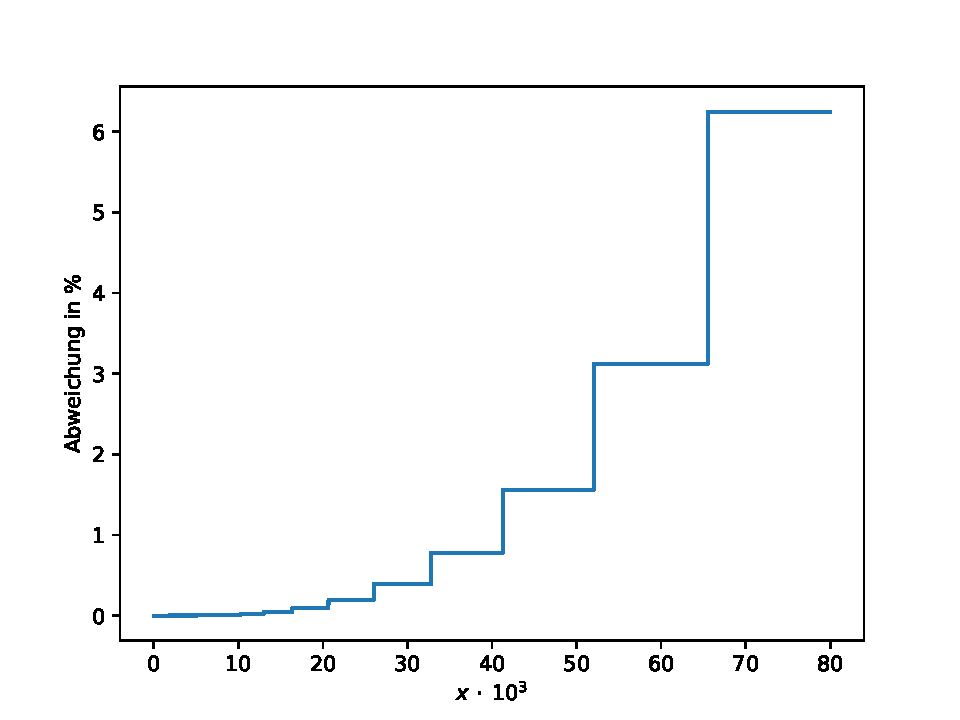
\includegraphics[width=\textwidth]{Aufgabe01/Fehler1a.pdf}
  \caption{Halblogarithmische Darstellung der Abweichung der Funktion \eqref{eqn:f}}
  \label{fig:1a}
\end{figure}

\begin{figure}[H]
  \centering
  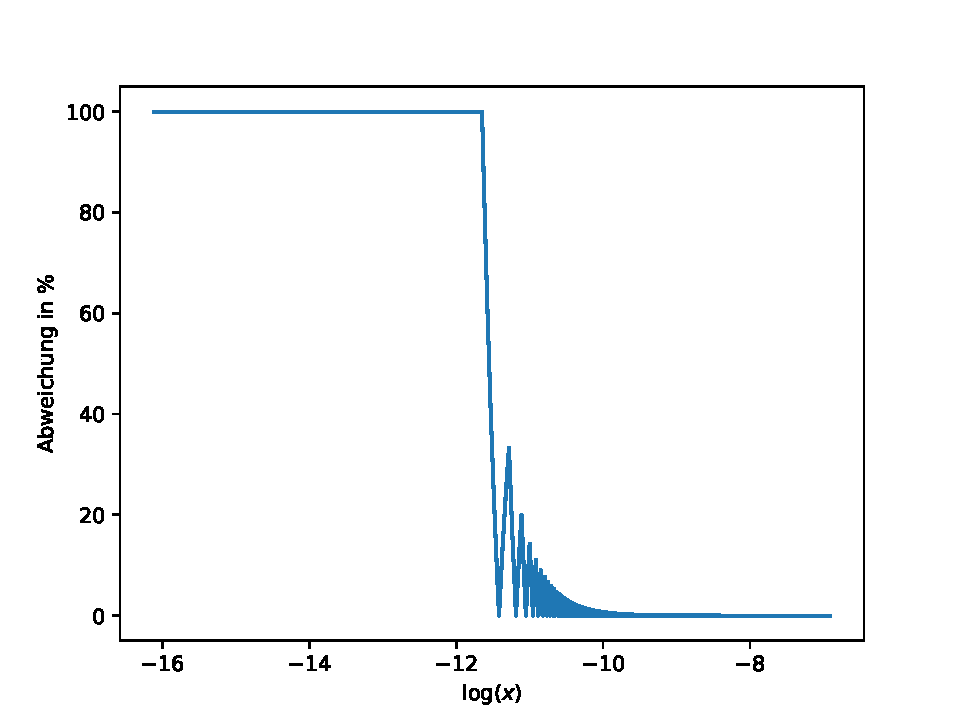
\includegraphics[width=\textwidth]{Aufgabe01/Fehler1b.pdf}
  \caption{Darstellung der Abweichung der Funktion \eqref{eqn:g}}
  \label{fig:1b}
\end{figure}
